% Intelligent Control System midterm proposal -- Team Charlie.
% The supplied ieeeconf.cls is retained unchanged.

% --- Document class and packages ---
\documentclass[letterpaper, 10 pt, conference]{ieeeconf}
\IEEEoverridecommandlockouts
\overrideIEEEmargins
\usepackage[utf8]{inputenc}
\usepackage[T1]{fontenc}
\usepackage{graphicx,amsmath,amssymb}
\usepackage{balance}
\usepackage{etoolbox}
\usepackage[hidelinks]{hyperref}
\usepackage{iftex}
\usepackage{zref-savepos}
\usepackage{zref-user}

% --- Checklist annotations: T1--T8, I1--I5, M1--M7 ---
% Position review icons in the outer page margins; they do not print.
% The Abstract heading is the parent of Problem/Solution/Contribution in
% guideline slide 6; those three are counted as T4/T5/T6.
\makeatletter
% Optional offset moves only the icon vertically, without changing the text.
\newcommand{\checkitem}[4][0pt]{%
  #4%
  \begingroup
  \pdfstringdef\reviewsubject{#2}%
  \pdfstringdef\reviewcontents{#2: #3}%
  \edef\reviewannotation{%
    /Subtype /Text /F 0 /Name /Comment
    
    /Subj (\reviewsubject)
    /Contents (\reviewcontents)}%
  \zsavepos{review-#2}%
  \dimen@=\zposx{review-#2}sp\relax
  \ifdim\dimen@<.5\paperwidth
    \dimen@ii=8pt\relax
  \else
    \dimen@ii=\dimexpr\paperwidth-24pt\relax
  \fi
  \advance\dimen@ii by -\dimen@
  \raisebox{#1}[0pt][0pt]{\hbox to 0pt{\kern\dimen@ii%
  \ifPDFTeX
    \pdfannot width 0pt height 0pt depth 0pt {\reviewannotation}%
  \else\ifLuaTeX
    \pdfextension annot width 0pt height 0pt depth 0pt {\reviewannotation}%
  \else
    \special{pdf:ann width 0pt height 0pt depth 0pt <<\reviewannotation>>}%
  \fi\fi
  \hss}}%
  \endgroup
}
\makeatother
\newcommand{\ThomasName}{Thomas Noirot}
\newcommand{\ThibaultName}{Thibault Lucas}

% --- Title and authors ---
\title{\LARGE\bf Predictive Coordination of Thrust and Moving Mass\\
for \checkitem{T1 Title}{Identifies predictive coordination of thrust and moving mass for underwater maneuvers.}{Underactuated Underwater Maneuvering}}
\author{\checkitem{T2 Authors}{Lists the authors and their affiliations.}{Sergi} Flores Mar\'in$^{1}$, \ThomasName$^{1}$, \ThibaultName$^{1}$, Takashi Arai$^{1}$, and Min-Fan Ricky Lee$^{2}$%
\thanks{$^{1}$Intelligent Control System course project, National Taiwan University of Science and Technology, Taipei, Taiwan.}%
\thanks{$^{2}$Graduate Institute of Automation and Control, National Taiwan University of Science and Technology, Taipei, Taiwan (e-mail: \texttt{rickylee@mail.ntust.edu.tw}).}%
}   

% --- Paper ---
\begin{document}
\maketitle
\thispagestyle{empty}
\pagestyle{empty}
% T1: title; T2: author block.

\begin{abstract}
We will design and build a low-cost underwater robot with two fixed horizontal thrusters and a longitudinal moving mass to change pitch. Changing depth requires tilting the body to redirect thrust, so combined turns and depth changes must account for the shared thrust and the time needed to move the \checkitem{T4 Abstract problem}{Turning and depth changes share limited thrust and require time to change pitch.}{mass.}
We will compare nonlinear model predictive control, which plans motor commands and mass motion together, with a cascade controller that also anticipates the reference and compensates for actuator response. Simulation will support development alongside construction, with prototype measurements used to refine simulation and prediction before selected pool \checkitem{T5 Abstract solution}{Proposes joint predictive control, supported by simulation, prototype measurements, and pool tests.}{tests.}
By testing turns and depth changes separately and together, we aim to determine whether joint prediction improves tracking and completion, while tests with currents, force pulses, and parameter uncertainty will assess robustness. If measurements justify a more detailed moving-mass model, we will test whether it improves \checkitem{T6 Abstract contribution}{Will evaluate the benefit of joint prediction and, if justified, a more detailed moving-mass model.}{control.}
\end{abstract}

\begin{keywords}
Model predictive control, moving-mass actuation, trajectory tracking, underactuated underwater \checkitem[-8pt]{T3 Keywords}{Four keywords identify the control method, actuation, task, and vehicle type.}{robots.}
\end{keywords}

\section{INTRODUCTION}

We plan to design and build a low-cost remotely operated vehicle (ROV), following the concept in Fig.~\ref{fig:concept}. Two independently driven, fixed horizontal thrusters will control forward motion and yaw, while a longitudinal moving mass will shift the center of gravity (CG) to change pitch. This will let the robot direct thrust upwards or downwards to change depth without a vertical \checkitem{I1 Problem}{The vehicle must coordinate thrust and moving-mass pitch control to combine turning and depth changes.}{thruster.}

% Queue the concept figure early so it occupies the first-page right column.
\begin{figure}[!t]
\centering
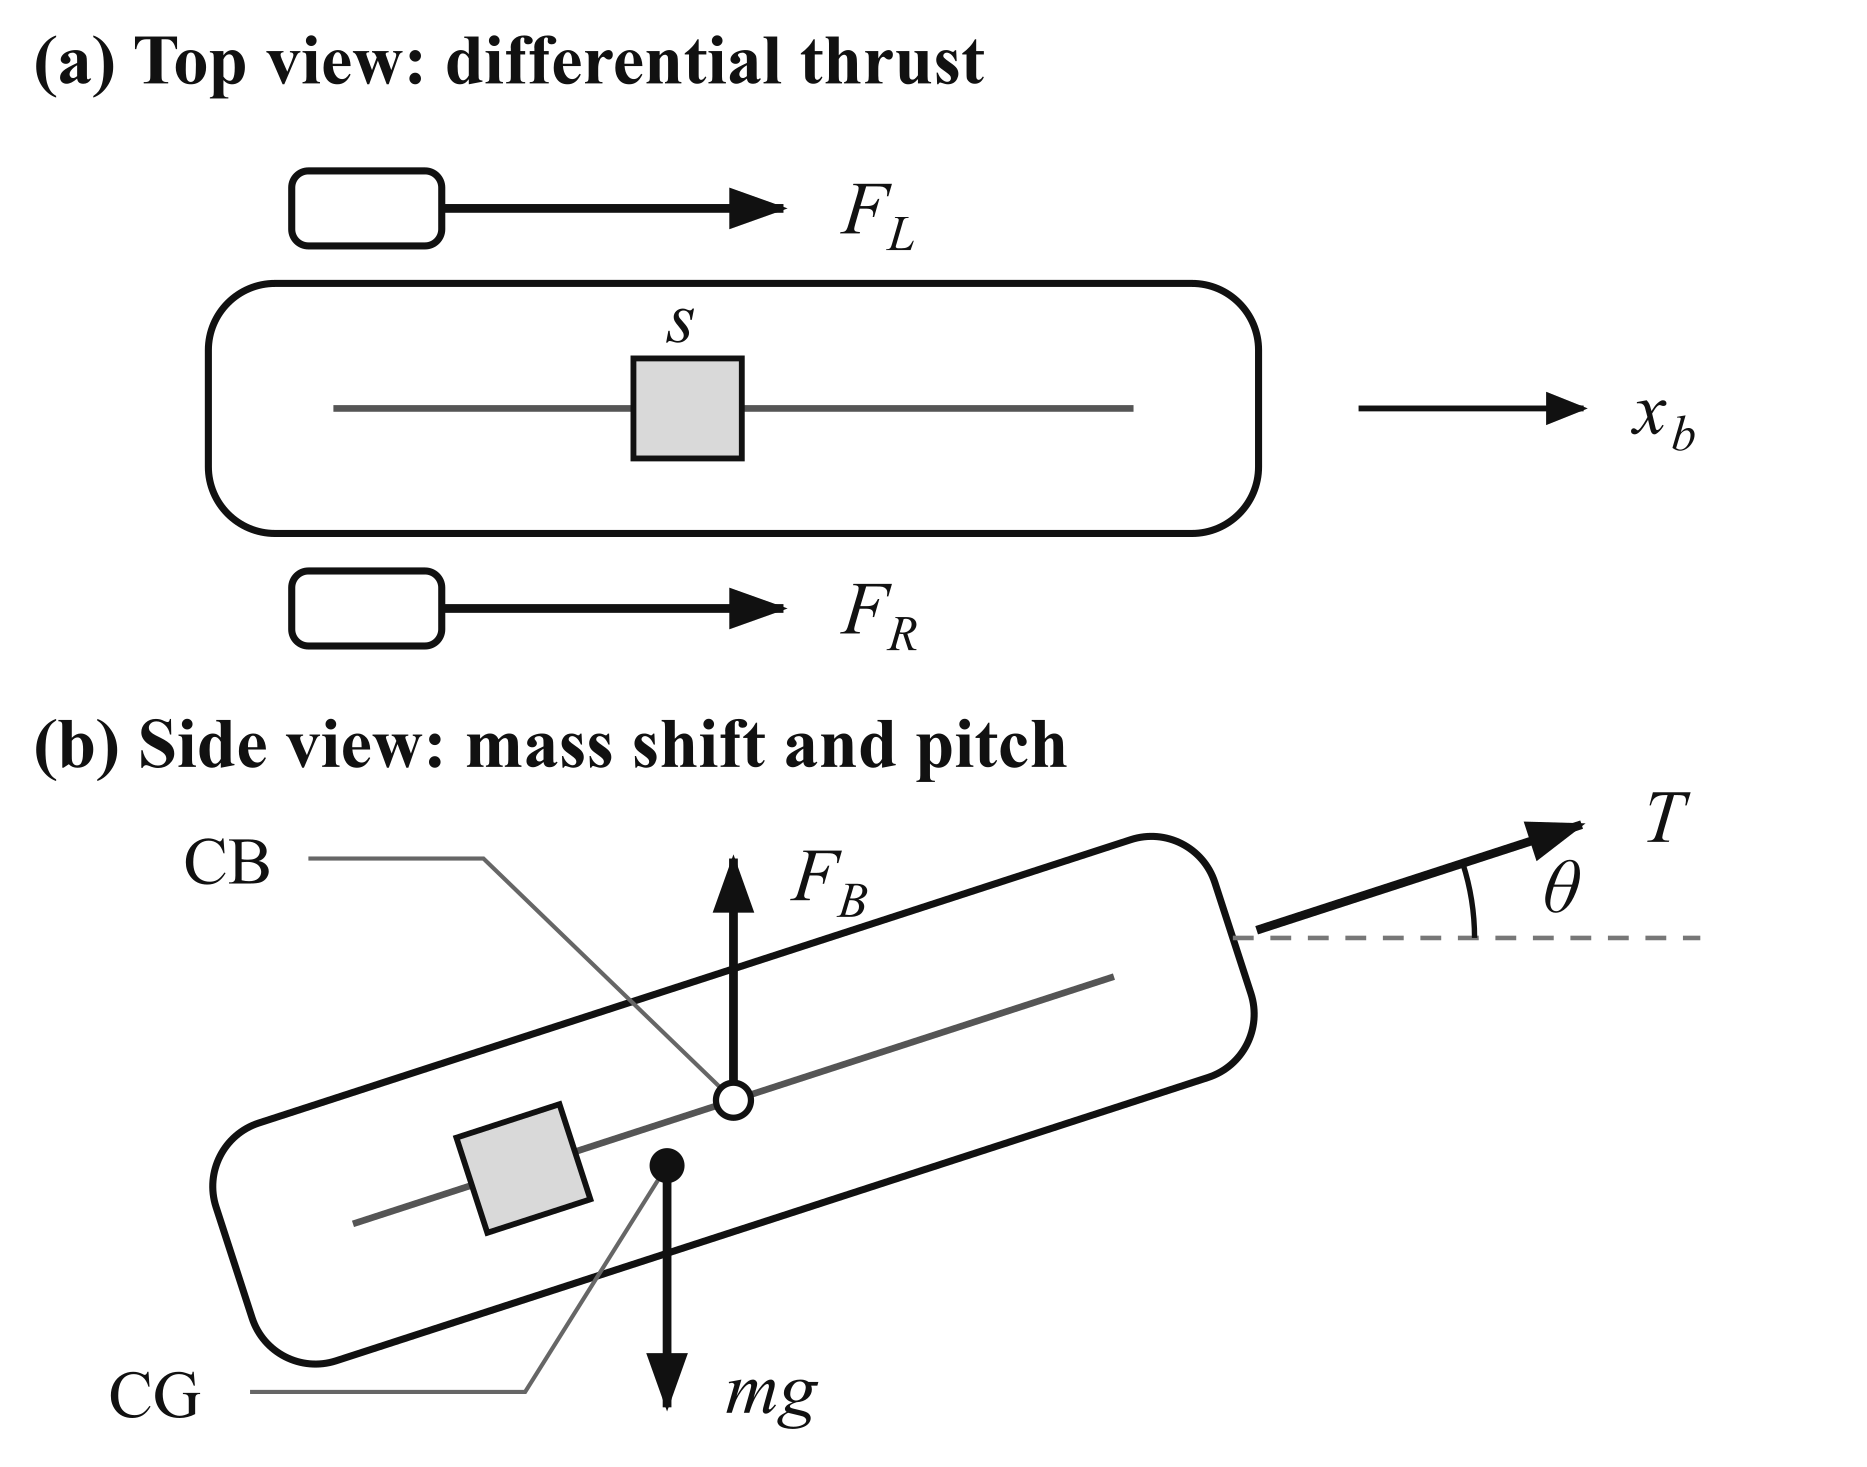
\includegraphics[width=0.895\columnwidth]{figures/rov_actuation.png}
\caption{Proposed actuation (not to scale). Carriage position $s$ shifts the center of gravity (CG) relative to the center of buoyancy (CB). Buoyancy $F_B$ and weight $mg$ produce a pitching moment; pitch $\theta$ redirects thrust $T$.}
\label{fig:concept}
\end{figure}

Using fewer actuators can simplify construction, but it also makes the timing of motor and mass commands more important. Tilting too late or using too much thrust to turn can prevent the robot from completing a maneuver, even with accurate external position \checkitem{I2 Importance}{Poor coordination can prevent maneuver completion even when accurate position measurements are available.}{measurements.}

Bhat \emph{et al.} evaluate nonlinear model predictive control (NMPC) in simulation and a linear time-varying variant experimentally on SAM, which combines thrust vectoring, variable buoyancy, and moving-mass trim~\cite{bhat}. Related work uses moving masses for depth control under uncertainty and constraints~\cite{chai}, or combines feedforward and feedback for glider motion~\cite{mahmoudian}. Closer to our motor layout, Muto \emph{et al.} simulate a vehicle with two orientable thrusters and an internal moving mass to compensate for pitch motion~\cite{muto}.

Zhong \emph{et al.} combine a quantized horizontal kinematic model with proportional--integral--derivative (PID) depth control~\cite{zhong}, assuming that speeds settle quickly and horizontal and vertical motion can be treated largely separately. In our vehicle, changing depth requires pitch to redirect the same thrust used for turning and following the \checkitem{I4 Findings extended}{Extends predictive maneuvering and moving-mass control to combined turns and depth changes with fixed thrusters.}{path.}

Building on these studies, we will test whether planning mass motion and thrust together improves combined turns and depth changes. We expect the greatest benefit when turns require high thrust and the robot has little time to change \checkitem{I3 Research gap}{Tests whether joint prediction improves combined maneuvers with fixed thrusters and moving-mass pitch control.}{pitch.} We will compare NMPC with a cascade controller that receives the same reference preview, using matched maneuvers and selected physical \checkitem[-6pt]{I5 Proposed solution}{Compares NMPC with an anticipatory cascade controller through matched maneuvers and selected pool tests.}{tests.}

\section{METHOD}

\subsection{Vehicle concept and parallel hardware development}

Before buying parts, we will prepare assembly drawings and a numbered bill of materials for the Safe Plan (approximately NT\$30,000) and Low-cost Plan. Both use the same actuation layout, with construction and electronics chosen for sealing, maintenance, cost, and local \checkitem{M1 Materials and overview}{Method A describes the two construction plans, components, actuation layout, and equipment source.}{availability.}

For longitudinal forces $F_L,F_R$ at body coordinates \mbox{$y_L=-b$}, \mbox{$y_R=b$},
\begin{equation}
T=F_L+F_R,\qquad \tau_z^b=b(F_L-F_R),
\end{equation}
where $\tau_z^b$ is the body-axis turning moment. A symmetric per-motor force limit $F_{\max}$ implies $|T|+|\tau_z^b|/b\leq2F_{\max}$. Actual thrust allocation will use measured forward and reverse limits. The vertical thrust has magnitude $|T\sin\theta|$, so changing depth depends on both pitch and the thrust available while the motors also generate a turning \checkitem{M2 Background}{The thrust equations explain why turning and depth changes compete for propulsion.}{moment.}

% Mechanical design.
Both the Safe Plan and Low-cost Plan share the frame, actuation, and internal layout. Two printed
cradles hold the hull in a PVC frame carrying the thrusters at CG height
($b=130$~mm), so thrust adds no pitching moment. Foam on the upper rails
and lead on the skids keep the center of buoyancy above the CG for roll
stability and allow external trimming. A 480~g lead carriage travels $\pm70$~mm on a NEMA17 lead screw between limit switches, for an estimated pitch of $\pm25^\circ$.

The plans differ in the pressure hull: the Safe Plan uses a Blue Robotics
101.6~mm (4 inches) inner diameter enclosure with a 400~mm acrylic tube, double radial O-ring flanges,
and penetrators~\cite{bluerobotics}, while the Low-cost Plan uses PVC pipe,
printed ABS end caps, and potted cable glands. Both will be vacuum tested
before each dive.

The electronics diagram of the robot can be divided in two subsystems: the control electronics (sensors and computing modules) and the power electronics (actuators and their power modulators). To avoid having important current surges from the power electronics (at motor start for example) disturbing or damaging the control electronics, two separate batteries are used, one for each subsystem.

Control electronics: The robot will include an IMU and a pressure sensor, with a camera for future projects. It will also include a voltage/current sensor to monitor each battery, and two limit switches for the mass translation system. The computation will be done using a Raspberry Pi 3B (to start with), as well as a micro-controller (an ESP32), used to generate the motor control signals. The two computation units and most sensors will be connected using an I2C bus, with an I2C multiplexer if there are address conflicts.

Power electronics: The robot contains three actuators: two DC motors for the thrusters and one stepper motor for the moving mass. The thrusters will use their integrated ESCs, controlled by PWM signals from the micro-controller, while the stepper motor will use a suitable driver.
The power distribution and exact connections will be detailed in an annex document, and will have to be adapted to the exact component models used.

\subsection{Simulation, observations, and identification}

During pool tests, we will estimate three-dimensional position from an overhead camera and a side camera, using inertial measurements for attitude. Before comparing controllers, we will check calibration, refraction, occlusion, synchronization, and measurement delay.

We will model the body and moving mass together in MuJoCo~\cite{todorov}, using Fossen's formulation for added inertia, Coriolis effects, damping, buoyancy, and motion relative to currents~\cite{fossen}. We will check the coupling between body and mass against a Lagrangian model~\cite{rambech} where the mass is small relative to the body and moves slowly.

Initial parameters will come from geometry and component data so simulation can begin before the prototype is ready. Once it is available, we will refine the simulation and controller model using measurements of mass, buoyancy, balance, motor response, drag, and carriage step responses and reversals under load, following the approach in~\cite{benzon}.

The carriage model will start with a first-order position response and command delay, with travel, speed, and acceleration limits enforced separately. We will add response states only if they improve predictions on validation runs, keeping complete runs separate for fitting, model selection, and final \checkitem{M3 Precise details}{Specifies identification measurements, carriage-response modeling, and separate fitting, validation, and evaluation runs.}{evaluation} so the same trajectory is not reused across stages.

We will check behavior at rest and during mass motion, and consistency across simulation time-steps, before using pool tests to assess prediction accuracy. Pool tests will take place with the robot fully submerged and away from walls to reduce their influence on the measurements.

\subsection{Predictive control and comparison}

The robot will follow a smooth three-dimensional (3D) position reference defined over time and within its motion limits. Orientation will follow from the predicted motion rather than a separate target. The model is
\begin{equation}
\hat x_{i+1}=f_{\vartheta}(\hat x_i,u_i),\qquad
u_i=(u_{L,i},u_{R,i},s_i^{\rm ref}),
\end{equation}
where $u_L,u_R$ are motor commands, $s^{\rm ref}$ the target carriage position, and $\vartheta$ fitted parameters. The state includes body pose and velocities, carriage position, and actuator-response states, estimated from current and past camera, inertial, and carriage measurements. Predictions include restoring moments as the CG moves and reactions from carriage motion, without advance knowledge of disturbances.

At each control step, NMPC minimizes
\begin{equation}
J=\sum_{i=0}^{N-1}\!\left(\|\hat p_i-p_i^\star\|_Q^2+\|\Delta u_i\|_R^2\right)
+\|\hat p_N-p_N^\star\|_{Q_f}^2,
\end{equation}
and applies the first command before receiving new measurements and replanning. Here $N$ is the horizon in samples, $\hat p_i$ predicted position, $p_i^\star$ the reference, and $Q,R,Q_f$ cost weights. The increment $\Delta u_i=u_i-u_{i-1}$ uses the previous command $u_{-1}$ at the first step. The controller plans pitch and thrust together so the mass can move before a depth change, while respecting actuator, depth, and attitude \checkitem{M4 Justification}{NMPC anticipates pitch preparation while coordinating thrust under actuator and operating limits.}{limits.}

For comparison, the cascade controller will combine position and velocity guidance with pitch and yaw PID, anti-windup, carriage control, and feasible thrust allocation, drawing on prior \checkitem{M6 Link to research}{The cascade baseline draws on the cited predictive and moving-mass control architectures.}{architectures}~\cite{bhat,chai,muto}. Feedforward and response compensation will help it prepare trim changes, using the same observations and reference preview as NMPC.

If measurements justify a detailed carriage model, we will compare both NMPC versions on moderate maneuvers and near actuator limits. Both will share body mechanics, motor dynamics, fitting data, cost, horizon, limits, and simulated robot, so only the carriage-response model changes.

We will test horizons around the measured pitch-response time, accounting for computation and command delays. If optimization takes too long, the robot will receive an alternative command within actuator limits.

\subsection{Experiments and evaluation}

The main experiment will compare depth reversals during straight motion, turns at constant depth, and their combination. By varying duration, curvature, and how much the maneuvers overlap, we will test whether joint prediction helps when pitch preparation and turning compete for \checkitem{M7 Crux}{Matched separate and combined maneuvers isolate when pitch preparation and turning compete for thrust.}{propulsion.} Final tests will use combinations not used for tuning, within measured actuator limits. A 3D helix will also show how the robot combines turning and depth changes continuously.

Completion rates will include all runs, with tracking errors compared on maneuvers both controllers complete. Alongside failures, we will report position root-mean-square error against the timed reference, maximum deviation, actuator saturation, and missed computation deadlines. Carriage, pitch, and thrust plots will help explain differences.

Preliminary runs will be used to tune the controllers and define success criteria. Final evaluation will use at least ten paired trials per condition, varying initial states, parameters, and noise between trials but matching them within each pair. Results will include paired differences and uncertainty intervals. For model comparisons, we will define an acceptable error margin in advance, so an uncertain result is not mistaken for equal performance.

Once the robot can follow the reference, we will introduce force pulses and measure the time needed to return below a fixed position-error tolerance and stay there for a specified duration. Runs that fail before a pulse will be reported separately. Further tests with uniform currents, parameter errors, and sensing and command delays will assess robustness without revealing disturbance schedules or the true parameters used in each simulation run.

After checking sealing, balance, and model predictions, pool tests will cover an easy maneuver and one where coordination should matter. We aim for five repetitions per controller, varying controller order. In push tests, we will record position and velocity when the push ends. Simulation provides an independent course deliverable, while conclusions about the real robot require physical \checkitem{M5 Caution}{Physical conclusions depend on pool tests following sealing, balance, and model checks.}{tests.}

Sergi handles writing, simulation, and control, while Thomas Noirot handles mechanics and Thibault handles electronics and sourcing. Takashi Arai provides guidance and coordinates reviews. We aim to finish drawings by November 2 and run a first pool test before November 7, depending on approval and parts availability. Software development will proceed alongside construction, with evaluation in November and final tests and reporting in December.

If model or computation limits affect NMPC, we may explore reinforcement learning in simulation as time allows. After meeting the single-vehicle goals, we may also simulate motion and tension control of two cable-connected ROVs.

% --- References ---
% Balance the final page without changing the supplied template margins.
\balance
% T7: references. Citation entries distinguish publications and preprints.

\begin{thebibliography}{99}
\bibitem{bhat} S. Bhat, C. Panteli, I. Stenius, and D. V. Dimarogonas, ``\checkitem{T7 References}{References support the related work and modeling choices; the preprint is identified as such.}{Nonlinear} model predictive control for hydrobatics: Experiments with an underactuated AUV,'' \emph{J. Field Robot.}, vol. 40, no. 7, pp. 1840--1859, 2023, doi: \href{https://doi.org/10.1002/rob.22218}{10.1002/rob.22218}.
\bibitem{chai} H. Chai, T. Zhang, and X. Yan, ``EKF-based adaptive integral MPC for depth control of an AUV under uncertainties and constraints,'' \emph{Ocean Eng.}, vol. 351, art. 124305, 2026, doi: \href{https://doi.org/10.1016/j.oceaneng.2026.124305}{10.1016/j.oceaneng.2026.124305}.
\bibitem{mahmoudian} N. Mahmoudian and C. A. Woolsey, ``An efficient motion control system for underwater gliders,'' \emph{Nonlinear Eng.}, vol. 2, no. 3--4, pp. 63--77, 2013, doi: \href{https://doi.org/10.1515/nleng-2012-0011}{10.1515/nleng-2012-0011}.
\bibitem{muto} K. Muto, T. Murakami, and E. Simetti, ``A PID-backstepping hybrid position and attitude control of a bi-copter AUV with a moving mass,'' in \emph{Proc. IEEE Int. Conf. Mechatronics}, 2025, doi: \href{https://doi.org/10.1109/ICM62621.2025.10934859}{10.1109/ICM62621.2025.10934859}.
\bibitem{zhong} Y. Zhong \emph{et al.}, ``Model predictive control with quantized inputs for three-dimensional trajectory tracking of a biomimetic electric ray,'' \emph{IEEE/ASME Trans. Mechatronics}, vol. 31, no. 4, pp. 4585--4593, 2026, doi: \href{https://doi.org/10.1109/TMECH.2026.3694472}{10.1109/TMECH.2026.3694472}.
\bibitem{bluerobotics} Blue Robotics, ``Watertight enclosure (WTE), 4-inch series,'' product documentation, 2026.
\bibitem{todorov} E. Todorov, T. Erez, and Y. Tassa, ``MuJoCo: A physics engine for model-based control,'' in \emph{Proc. IEEE/RSJ Int. Conf. Intell. Robots Syst.}, 2012, pp. 5026--5033, doi: \href{https://doi.org/10.1109/IROS.2012.6386109}{10.1109/IROS.2012.6386109}.
\bibitem{fossen} T. I. Fossen, \emph{Handbook of Marine Craft Hydrodynamics and Motion Control}, 2nd ed. Wiley, 2021.
\bibitem{rambech} A. B. Rambech, I. B. Saksvik, and V. Hassani, ``Combining moving mass actuators and manoeuvring models for underwater vehicles: A Lagrangian approach,'' arXiv:2510.25479, 2025.
\bibitem{benzon} M. von Benzon \emph{et al.}, ``An open-source benchmark simulator: Control of a BlueROV2 underwater robot,'' \emph{J. Mar. Sci. Eng.}, vol. 10, no. 12, art. 1898, 2022, doi: \href{https://doi.org/10.3390/jmse10121898}{10.3390/jmse10121898}.
\end{thebibliography}

% --- Author biographies ---
\section*{AUTHOR BIOGRAPHIES}

% Keep fixed biography spacing and reserve room for the photographs.
\makeatletter
\expandafter\patchcmd\csname\string\biography\endcsname{\vskip \@IEEEBIOskipN plus 1fil minus 0\baselineskip}{\vskip \@IEEEBIOskipN}{}{\PackageError{Biography spacing}{Could not adjust biography spacing}{Check the biography environment.}}
\def\@IEEEBIOskipN{0.7\baselineskip}
\def\@IEEEBIOhangdepth{1.0in}
\makeatother
\begingroup
\normalfont\footnotesize
\interlinepenalty500
\setlength{\parskip}{0.7\baselineskip}
\begin{biography}[{\raisebox{0.14in}[\height][\depth]{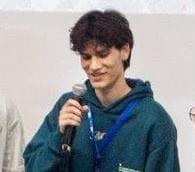
\includegraphics[width=1.10in,keepaspectratio]{Author Photo/sergi_photo_paper.jpeg}}}]{Sergi Flores Mar\'in}
is a final-year Artificial Intelligence student at the Universitat Polit\`ecnica de Catalunya (UPC), currently on exchange at the National Taiwan University of Science and Technology (NTUST). His research experience at the Institut de Rob\`otica i Inform\`atica Industrial (IRI) includes diffusion policies and reinforcement learning for quadruped locomotion.\checkitem{T8 Biographies}{Biographies describe the authors’ education and research backgrounds.}{}
\end{biography}

\begin{biography}[{\raisebox{0.14in}[\height][\depth]{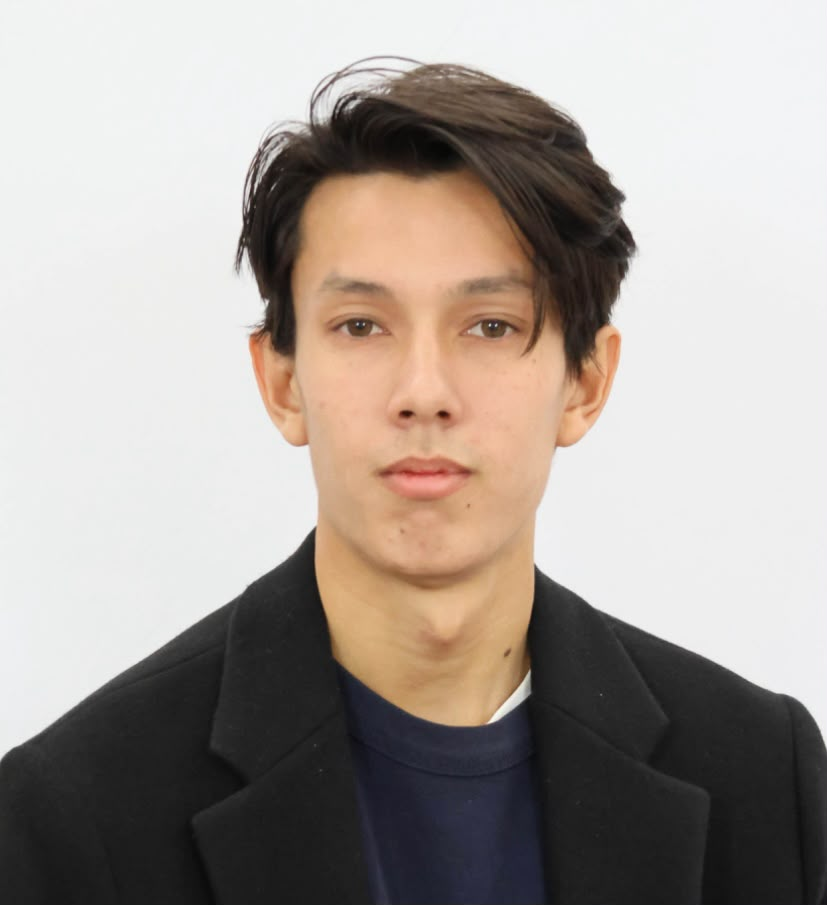
\includegraphics[width=1.10in,trim=0 175bp 0 0,clip]{Author Photo/Thomas.jpeg}}}]{Thomas Noirot}
completed his CPGE in Physics and Engineering Science at Jules Garnier, New Caledonia, in 2024. He is pursuing a Master's in Mechanical Engineering at SIGMA Clermont, France, specializing in Innovative Mechanisms and Robotics, and is on exchange at NTUST, Taiwan. His research focuses on digital twins, and his interests include robotics for manufacturing.
\end{biography}

\makeatletter
\def\@IEEEBIOphotowidth{1.10in}
\def\@IEEEBIOphotodepth{0.74in}
\def\@IEEEBIOhangwidth{1.14in}
\def\@IEEEBIOhangdepth{1.05in}
\def\@IEEEBIOskipN{0.7\baselineskip}
\makeatother
\begin{biography}[{\raisebox{-0.08in}[\height][\depth]{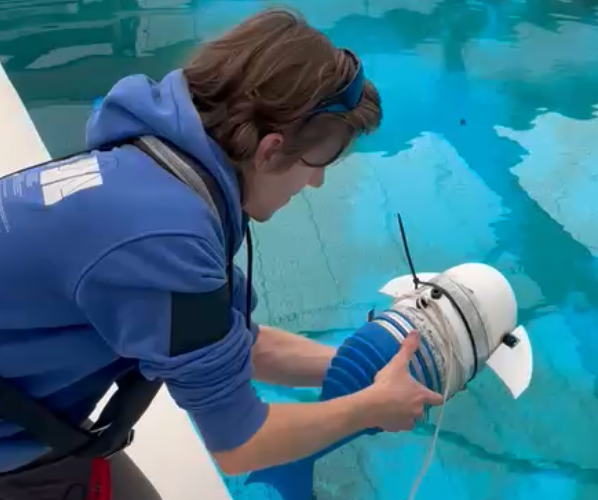
\includegraphics[width=1.1in,keepaspectratio]{Author Photo/thibault2.png}}}]{Thibault Lucas}
is a final-year graduate student at École Nationale Supérieure de Techniques Avancées (ENSTA), France, specializing in Autonomous Robotics. He is on exchange at the National Taiwan University of Science and Technology (NTUST), Taiwan. His research projects and interests revolve around the design of robotic systems evolving in constrained environments.
\end{biography}

% Takashi Arai.
\makeatletter
\def\@IEEEBIOphotowidth{1.10in}
\def\@IEEEBIOphotodepth{0.74in}
\def\@IEEEBIOhangwidth{1.14in}
\def\@IEEEBIOhangdepth{1.05in}
\def\@IEEEBIOskipN{0.7\baselineskip}
\makeatother
\begin{biography}[{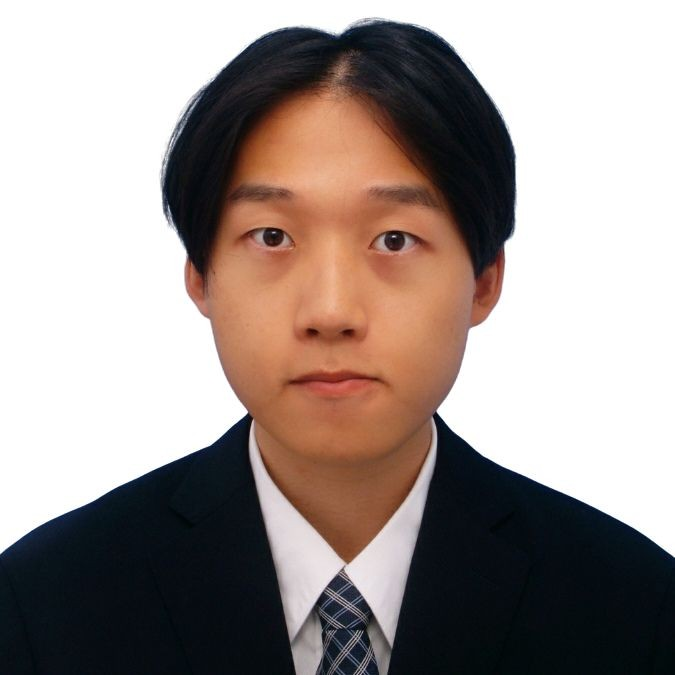
\includegraphics[width=1.1in,keepaspectratio]{Author Photo/Taka1.jpeg}}]{Takashi Arai}
is a master's student in the Computer Science and Intelligent Systems Program at the University of the Ryukyus, Japan. He is currently an exchange student at the National Taiwan University of Science and Technology (NTUST), Taiwan. His research focuses on cooperative control of multiple underwater robots.
\end{biography}
\par\endgroup

% Professor biography and photograph.
\makeatletter
\def\@IEEEBIOphotowidth{1.10in}
\def\@IEEEBIOphotodepth{0.74in}
\def\@IEEEBIOhangwidth{1.25in}
\def\@IEEEBIOhangdepth{0.76in}
\def\@IEEEBIOskipN{0.7\baselineskip}
\makeatother
\begin{biography}[{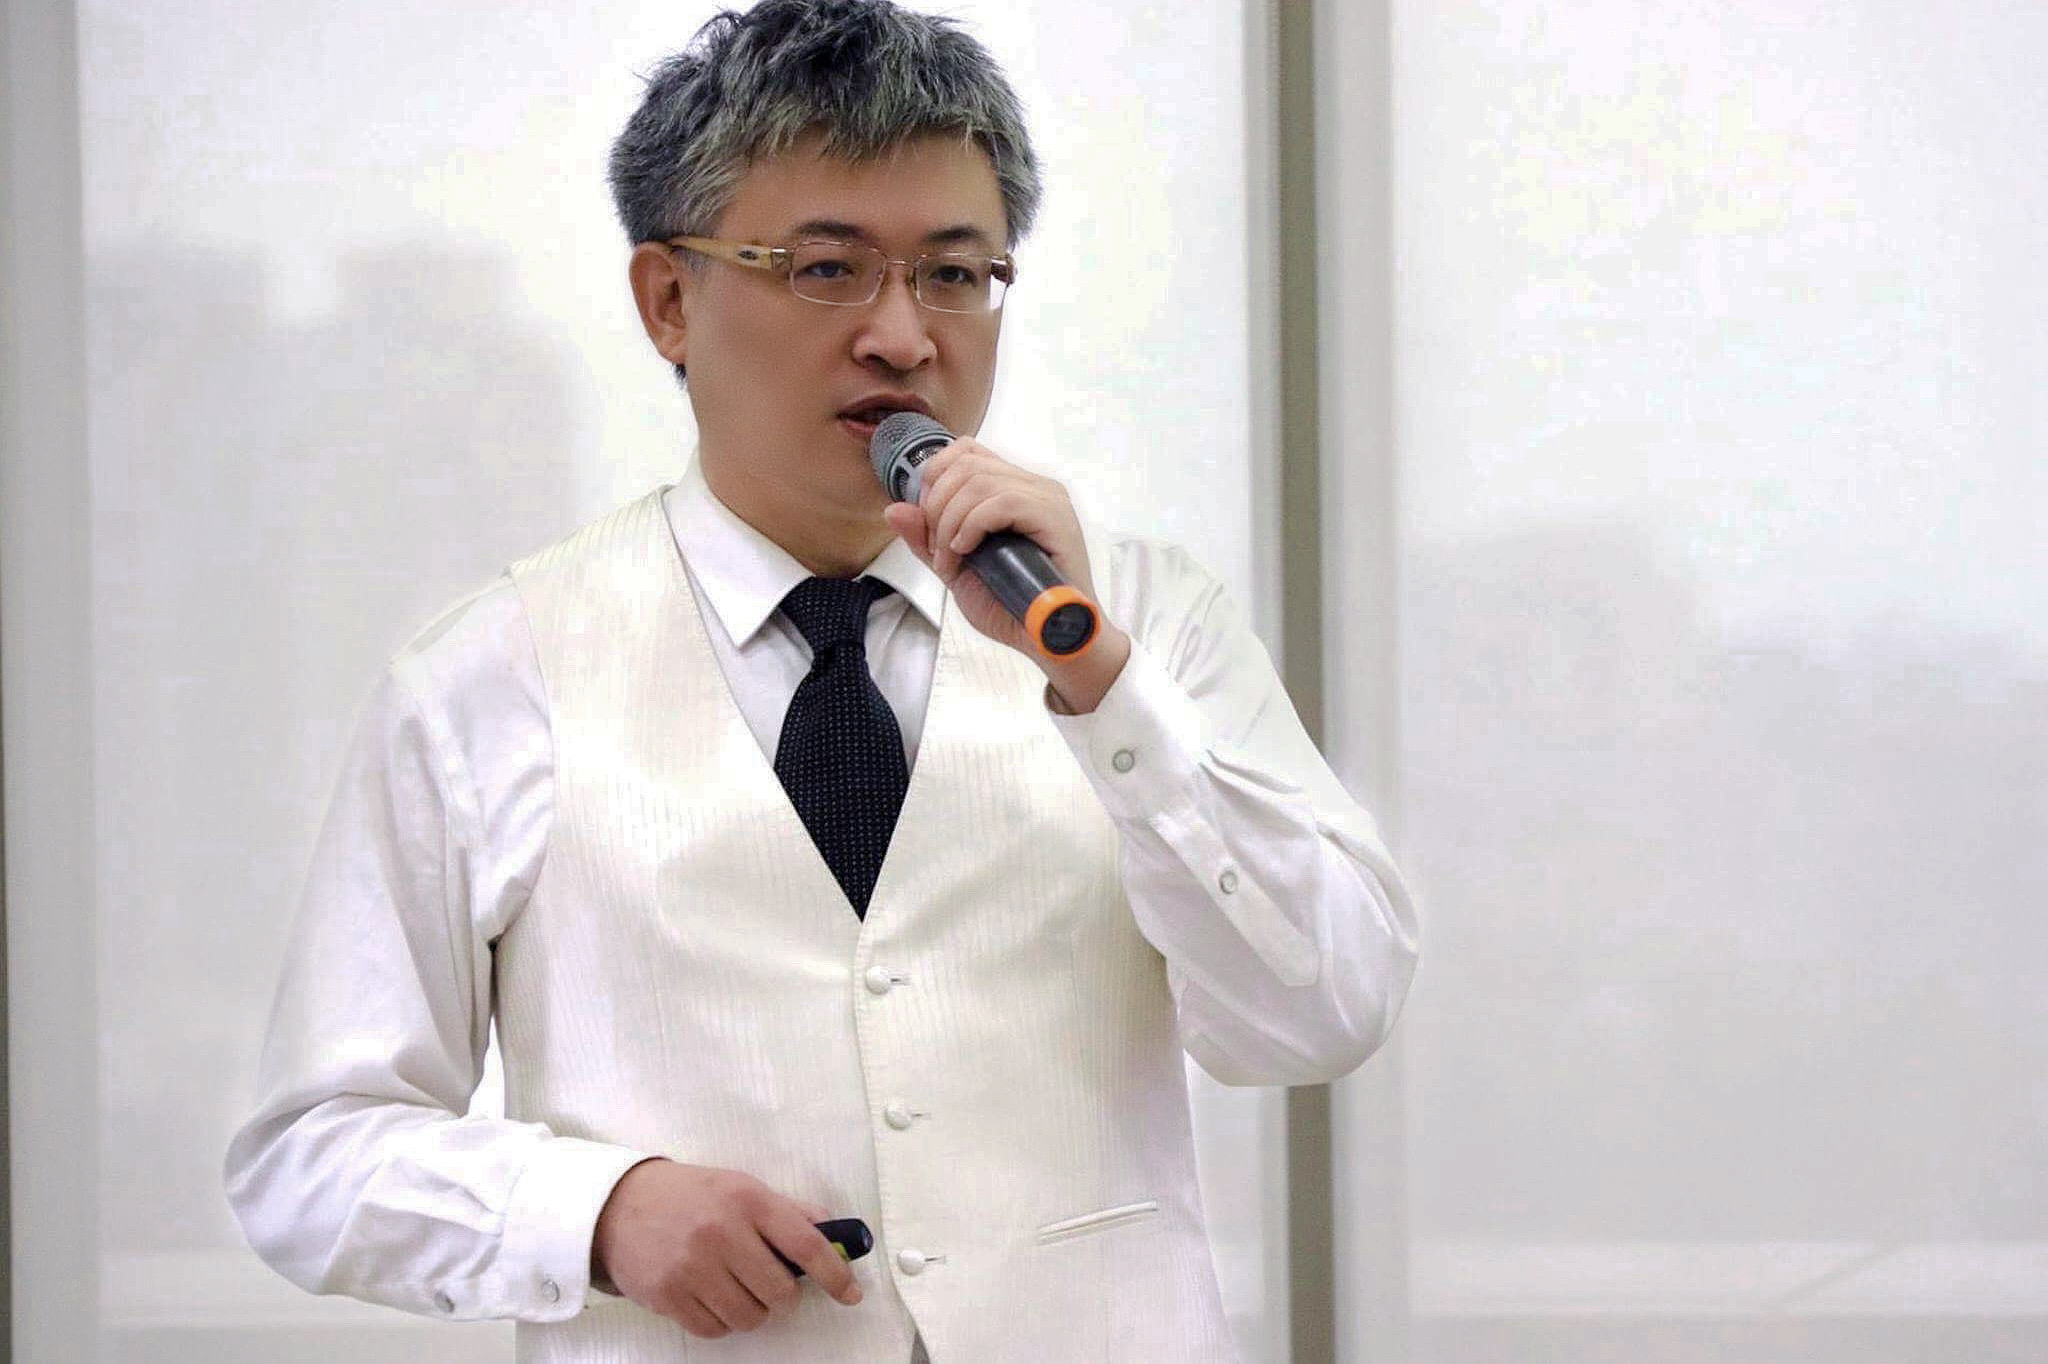
\includegraphics[width=1.10in,keepaspectratio]{Author Photo/Min-Fan Ricky Lee.JPG}}]{Min-Fan Ricky Lee}
received his B.S. from Tam Kang University, Taiwan, in 1988, and his M.S. and Ph.D. from Cornell University, USA, in 1991 and 1996. He is an Associate Professor at the Graduate Institute of Automation and Control, NTUST, Taiwan. He previously worked as a Research Scientist at the University of British Columbia (1996--1998) and a Research Officer at the National Research Council of Canada (1998--2007).
\end{biography}

\end{document}